 make -j eval-unblinder.exe && ./eval-unblinder.exe net.val
.!Evaluating model net.val...
Loaded 50000 positions in 122.59s
Loaded model in 0.10s
Ran eval in 2.04s
Reading [net.val]
net.val: 4 layers.
net.val: num nodes: 64 1024 12288 567 837
net.val: indices per node/fns: 49 LEAKY_RELU 36 LEAKY_RELU 127 LEAKY_RELU 78 LEAKY_RELU
Read from net.val.
Invert index:
Check it:
ModelInfo [339885 rounds, 223224128 examples]
Over 50000 positions:
  9584 exactly correct (19.17%)
  161166 piece mistakes (3.22/pos)
  1630 castling mistakes (0.03/pos)
  19014 move mistakes (0.38/pos)
  181810 total mistakes (3.64/pos)

$ make -j eval-unblinder.exe && ./eval-unblinder.exe net-before-vacuum.val
make: 'eval-unblinder.exe' is up to date.
Evaluating model net-before-vacuum.val...
Loaded 50000 positions in 118.80s
Loaded model in 3.99s
Ran eval in 332.10s
Reading [net-before-vacuum.val]
net-before-vacuum.val: 4 layers.
net-before-vacuum.val: num nodes: 64 1024 12288 567 837
net-before-vacuum.val: indices per node/fns: 64 LEAKY_RELU 1024 LEAKY_RELU 12288 LEAKY_RELU 567 LEAKY_RELU
Read from net-before-vacuum.val.
Invert index:
Check it:
ModelInfo [146999 rounds, 9407936 examples]
Over 50000 positions:
  10601 exactly correct (21.20%)
  156052 piece mistakes (3.12/pos)
  1542 castling mistakes (0.03/pos)
  18818 move mistakes (0.38/pos)
  176412 total mistakes (3.53/pos)



without concurrent processes:
net.val: 1.61s  (something like 1035/sec/core)
net-before-vacuum: 229.85s (something like 7/sec/core)


single_kings net.val:
Over 50000 positions:
  9642 exactly correct (19.28%)
  162804 piece mistakes (3.26/pos)
  1633 castling mistakes (0.03/pos)
  19014 move mistakes (0.38/pos)
  183451 total mistakes (3.67/pos)

It's actually kind of heartening that it performs worse with this approach,
though we are more likely to get the whole board correct.

(cite #kingme)


% all bits set to 1 (with single_kings)
% (without single_kings, only difference is that the bottom right becomes a
% rook; no white queen)
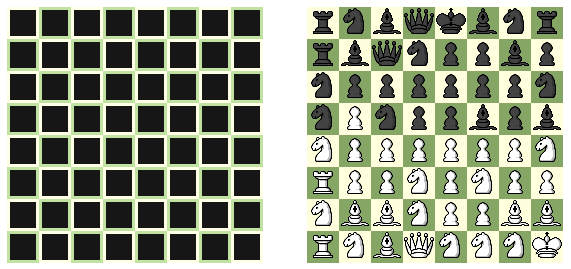
\includegraphics{allon}

